\documentclass{article}
\usepackage[a4paper, top=3cm, left=3cm, bottom=3cm, right=3cm]{geometry}
\usepackage[T1]{fontenc} 
\usepackage[utf8]{inputenc} 
\usepackage[italian]{babel} 
\usepackage{lipsum} 
\usepackage{url} 
\usepackage{lmodern}
\usepackage{graphicx}
\usepackage{psfrag}
\usepackage{amsfonts}
\usepackage{amsthm}
\usepackage{amsmath}
\usepackage{amssymb}
\usepackage{mathrsfs}
\usepackage{tikz-cd}
\usepackage{mathtools}
\usepackage{tikz} 
\usepackage{caption}
\captionsetup{labelformat=empty,textfont=sl}
\usetikzlibrary{decorations.markings}
\usepackage{enumitem}
\usepackage[hidelinks]{hyperref}
\usepackage[numbered,framed]{matlab-prettifier}

\lstset{
  style              = Matlab-editor,
  basicstyle         = \mlttfamily,
  escapechar         = ",
  mlshowsectionrules = true,
}

\title{\textbf{Laboratorio Sperimentale di Matematica Computazionale / / Spirale di Primi - B5}}
\author{Dario Rancati - 539365} 


\begin{document}

\maketitle

\noindent
Per individuare i primi nella distribuzione spiraleggiante dell'esercizio B5 ci serve innanzitutto una function che disegni questa distribuzione in funzione del lato $m$ della tabella, nel testo 500. Essa è la seguente

\begin{lstlisting}
function s = spiraleB5(m)
    s = zeros(m);
    %variabili posizioni e entrata 
    %settate ai valori iniziali
    i=1;
    j=1;
    k=1;
    s(i,j)=k;
    %ora iniziamo a girare
    for giri = 1:m-1;
        k=k+1;
        j=i+1;
        i=1;
        s(i,j)=k;
        %ora scendiamo
        for t = 1:giri
            k=k+1;
            i=i+1;
            s(i,j)=k;
        end
        %ora andiamo a sinistra
        for t = 1:giri
            k=k+1;
            j=j-1;
            s(i,j)=k;
        end    
    end
end   
\end{lstlisting}

\noindent
Adesso adottiamo il secondo metodo mostrato nelle slides, ossia usiamo la funzione \texttt{crivello} fornita nel testo per costruire la seguente function:

\begin{lstlisting}
function z = spiraleprimi(n)
s = spiraleB5(n);
m = max(max(s));
c = crivello(m);
z = c(s);
imshow(1 + z, [1 1 1 ; 0 0 1]);
\end{lstlisting}
\noindent
A questo punto il comando \texttt{spiraleprimi(500)} fornisce la seguente immagine, nella quale oltre all'addensamento sulle diagonali a $45°$ notiamo anche un addensamento sulle linee verticali e orizzontali:
\begin{figure}[h!]
\centering
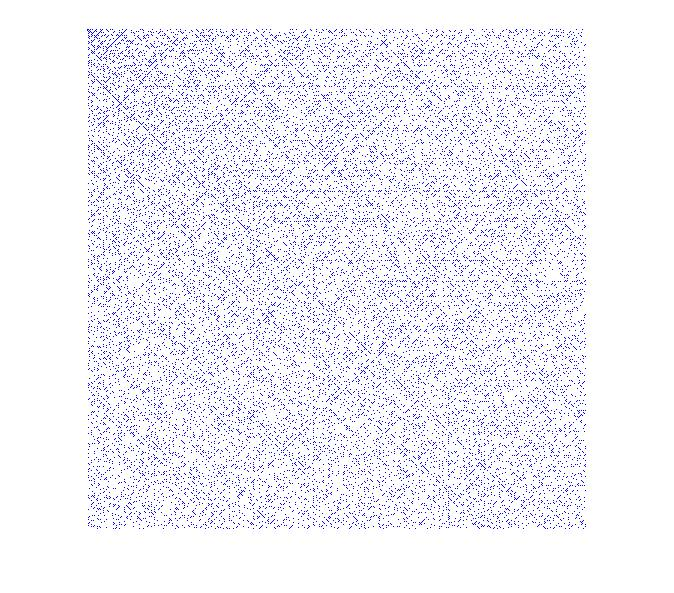
\includegraphics[width=\textwidth]{figura_B5.jpg}
\end{figure}

\end{document}